\section{eo\-Stat\-Base$<$ EOT $>$ Class Template Reference}
\label{classeo_stat_base}\index{eoStatBase@{eoStatBase}}
Base class for all statistics that need to be calculated over the (unsorted) population (I guess it is not really necessary? MS.  


{\tt \#include $<$eo\-Stat.h$>$}

Inheritance diagram for eo\-Stat\-Base$<$ EOT $>$::\begin{figure}[H]
\begin{center}
\leavevmode
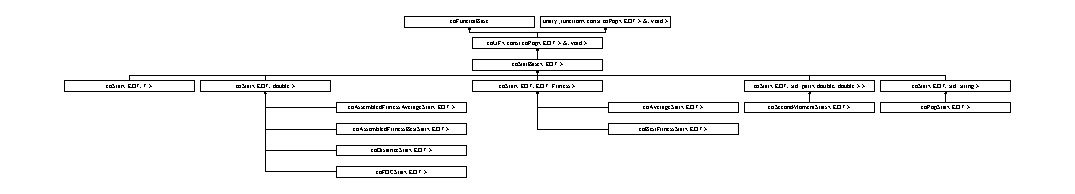
\includegraphics[height=2.16216cm]{classeo_stat_base}
\end{center}
\end{figure}
\subsection*{Public Member Functions}
\begin{CompactItemize}
\item 
virtual void {\bf last\-Call} (const {\bf eo\-Pop}$<$ {\bf EOT} $>$ \&)\label{classeo_stat_base_a0}

\item 
virtual std::string {\bf class\-Name} (void) const \label{classeo_stat_base_a1}

\end{CompactItemize}


\subsection{Detailed Description}
\subsubsection*{template$<$class EOT$>$ class eo\-Stat\-Base$<$ EOT $>$}

Base class for all statistics that need to be calculated over the (unsorted) population (I guess it is not really necessary? MS. 

Depstd::ends, there might be reasons to have a stat that is not an {\bf eo\-Value\-Param}{\rm (p.\,\pageref{classeo_value_param})}, but maybe I'm just kidding myself, MK) 



Definition at line 45 of file eo\-Stat.h.

The documentation for this class was generated from the following file:\begin{CompactItemize}
\item 
eo\-Stat.h\end{CompactItemize}
